\documentclass[final]{siamltexmm}
\documentclass[10pt,a4paper]{article}

\usepackage{graphicx}
\usepackage{algorithm}
\usepackage{algorithmic}

% \usepackage[demo]{graphicx}
% \usepackage{subfig}

\newcommand{\pe}{\psi}
\def\d{\delta} 
\def\ds{\displaystyle} 
\def\e{{\epsilon}} 
\def\eb{\bar{\eta}}  
\def\enorm#1{\|#1\|_2} 
\def\Fp{F^\prime}  
\def\fishpack{{FISHPACK}} 
\def\fortran{{FORTRAN}} 
\def\gmres{{GMRES}} 
\def\gmresm{{\rm GMRES($m$)}} 
\def\Kc{{\cal K}} 
\def\norm#1{\|#1\|} 
\def\wb{{\bar w}} 
\def\zb{{\bar z}} 

% some definitions of bold math italics to make typing easier.
% They are used in the corollary.

\def\bfE{\mbox{\boldmath$E$}}
\def\bfG{\mbox{\boldmath$G$}}

\title{Independent Study}
\author{Yun-shao Sung\thanks{\tt yss265@nyu.edu} }

\begin{document}
\maketitle

\begin{abstract}
This is independent study mid-way report
\end{abstract}

\pagestyle{myheadings}
\thispagestyle{plain}

\section{Abstract}
Hi1!

\\
\section{Introduction}
Hi2!

\\
\section{Baseline Approach}
Here is the baseline approach which can be roughtly divided into two parts: the first part is constructing symmetric matrix from the feature similarity along time, and the second part is to construct symmetric normalized Laplacian matrix and obtain the top $m$ eigenvectors with the top $m$ smallest eigenvalues, and then perform k-means for boundary detection.

\begin{algorithm}[htb]
  \caption{Baseline Approach}
  \SetKwInOut{Input: }{number of top $m$ smallest eigenvalues}
  \label{algo:SC}
\begin{algorithmic}[1]
  \STATE M = getSymmetricMatrix()
  \STATE L = scipy.sparse.csgraph.laplacian()
  \STATE eigVals, eigVecs = np.linalg.eig(L)
  \STATE Y = getMthSmallest(eigVals, eigVecs, m)
\end{algorithmic}
\end{algorithm}

\begin{algorithm}[htb]
  \caption{boundaryDetection}
  \SetKwInOut{Input: }{Laplacian eigenvectors $Y \in \mathbb{R^{n \times m}}$}

  \SetKwInOut{Output: }{Boundary b, Centroids c}
  \label{algo:SC}
\begin{algorithmic}[1]
  \STATE M = getSymmetricMatrix()
  \STATE L = scipy.sparse.csgraph.laplacian()
  \STATE eigVals, eigVecs = np.linalg.eig(L)
  \STATE Y = getMthSmallest(eigVals, eigVecs, m)
\end{algorithmic}
\end{algorithm}

\subsection{Hi2sub}
Hi2sub!

\begin{figure}[H]
  \centering
    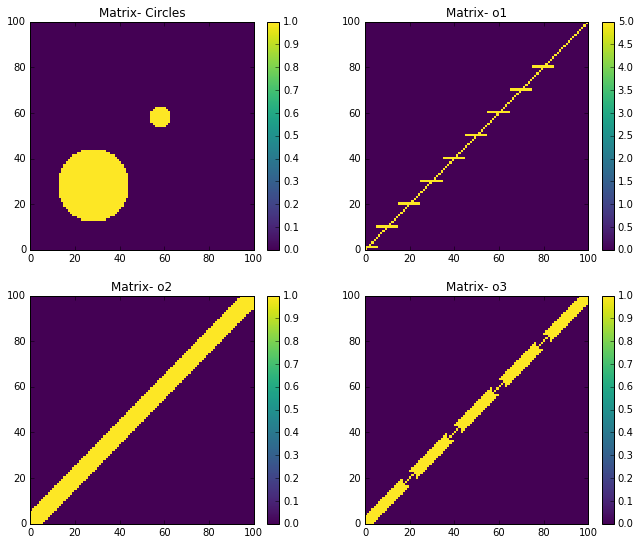
\includegraphics[width=0.5\textwidth]{./figure/similarityMatrix.png}
  \caption{The training and test accuracy with epochs}
\end{figure}


\subsection{ToDos}
Hi3!

\begin{thebibliography}{10}
\bibitem{fpf} {\sc A Tutorial on Spectral Clustering}
\bibitem{fpf} {\sc Analyzing Song Structure with Spectral Clustering}
\bibitem{fpf} {\sc Deep clustering: Discriminative embeddings for
segmentation and separation}
\bibitem{fpf} {\sc Learning Deep Representations for Graph Clustering}
\bibitem{fpf} {\sc Hierarchical Evaluation of Segment Boundary Detection}
\end{thebibliography}

\end{document}
